% (C) Brett Klamer - MIT - http://opensource.org/licenses/MIT
% Please contact me if you find any errors or make improvements
% Contact details at brettklamer.com

\documentclass[11pt,letterpaper,english,oneside]{article} % article class is a standard class
%==============================================================================
%Load Packages
%==============================================================================
\usepackage[left=1in,right=1in,top=1in,bottom=1in]{geometry} % easy page margins
\usepackage[utf8]{inputenc} % editor uses utf-8 encoding
\usepackage[T1]{fontenc} % T1 font pdf output
\usepackage{lmodern} % Latin modern roman font
\usepackage{bm, bbm} % bold and blackboard bold math symbols
\usepackage{amsmath, amsfonts, amssymb, amsthm} % math packages
\usepackage[final]{microtype} % better microtypography
\usepackage{graphicx} % for easier grahics handling
\usepackage[hidelinks, colorlinks=true, linkcolor = blue, urlcolor = blue]{hyperref} % to create hyperlinks
\usepackage{float} % tells floats to stay [H]ere!
\usepackage{enumitem} % nice lists
\usepackage{fancyhdr} % nice headers
\usepackage{caption}  % to control figure and table captions
\usepackage{booktabs} % to create nice tables

\captionsetup{width=0.9\textwidth, justification = raggedright}

%==============================================================================
% Enter name and homework title here
%==============================================================================
\author{Eugene Katsevich}
\title{Sample Homework}
\date{August 18, 2022}

%==============================================================================
% Put title and author in PDF properties
%==============================================================================
\makeatletter % change interpretation of @
\hypersetup{pdftitle={\@title},pdfauthor={\@author}}


%==============================================================================
% Header settings
%==============================================================================
\pagestyle{fancy} % turns on fancy header styles
\fancyhf{} % clear all header and footer fields
\makeatletter
\lhead{\@author} % left header
\chead{\@title} % center header
\makeatother
\rhead{Page \thepage} % right header
\setlength{\headheight}{13.6pt} % fixes minor warning
\makeatother % change back interpretation of @

%==============================================================================
% List spacing
%==============================================================================
\setlist[itemize]{parsep=0em} % fix itemize spacing
\setlist[enumerate]{parsep=0em} % fix enumerate spacing

%==============================================================================
% Float spacing (changes spacing of tables, graphs, etc)
%==============================================================================
%\setlength{\textfloatsep}{3pt}
%\setlength{\intextsep}{3pt}

%==============================================================================
% Define Problem and Solution Environments
%==============================================================================
\theoremstyle{definition} % use definition's look
\newtheorem{problem}{Problem}
\newtheorem{solution}{Solution}
\newenvironment{prob}{\clearpage \begin{problem}\hspace{0pt}}{\end{problem}}
\newenvironment{sol}{\begin{solution}\hspace{0pt}}{\end{solution}}

\begin{document}


\maketitle

\section{Instructions}

\paragraph{Setup.} Pull the latest version of this assignment from Github and set your working directory to \texttt{stat-961-fall-2021/homework/homework-1}. Consult the \href{https://github.com/Katsevich-Teaching/stat-961-fall-2021/blob/main/getting-started/getting-started.pdf}{getting started guide} if you need to brush up on \texttt{R}, \texttt{LaTeX}, or \texttt{Git}.

\paragraph{Collaboration.} The collaboration policy is as stated on the Syllabus:

\begin{quote}
``Students are permitted to work together on homework assignments, but solutions must be written up and submitted individually. Students must disclose any sources of assistance they received; furthermore, they are prohibited from verbatim copying from any source and from consulting solutions to problems that may be available online and/or from past iterations of the course.''
\end{quote}

\noindent In accordance with this policy, \\

\noindent \textit{Please list anyone you discussed this homework with:} I did not discuss this homework with anyone.

\paragraph{Writeup.} Use this document as a starting point for your writeup, adding your solutions between \verb|\begin{sol}| and \verb|\end{sol}|. See the \href{https://github.com/Katsevich-Teaching/stat-961-fall-2021/blob/main/getting-started/preparing-reports.pdf}{preparing reports guide} for guidance on compilation, creation of figures and tables, and presentation quality. Show all the code you wrote to produce your numerical results, and include complete derivations typeset in LaTeX for the mathematical questions. 

\paragraph{Programming.}

The \texttt{tidyverse} paradigm for data manipulation (\texttt{dplyr}) and plotting (\texttt{ggplot2}) are strongly encouraged, but points will not be deducted for using base \texttt{R}. 

\paragraph{Grading.} Each sub-part of each problem will be worth 3 points: 0 points for no solution or completely wrong solution; 1 point for some progress; 2 points for a mostly correct solution; 3 points for a complete and correct solution modulo small flaws. The presentation quality of the solution for each problem (as exemplified by the guidelines in Section 3 of the \href{https://github.com/Katsevich-Teaching/stat-961-fall-2021/blob/main/getting-started/preparing-reports.pdf}{preparing reports guide}) will be evaluated out of an additional 3 points.

\paragraph{Submission.} Compile your writeup to PDF and submit to \href{https://www.gradescope.com/courses/284562}{Gradescope}.

\clearpage

\begin{prob} \textbf{Quadratic theorem.} \\

\noindent Consider a right triangle with legs of lengths $a$ and $b$ and hypotenuse of length $c$. 
\begin{enumerate}
\item[(a)] State the Pythagorean theorem.
\item[(b)] Who initially proposed this theorem?
\end{enumerate}

\end{prob}

\begin{sol}

\begin{enumerate}
  \item[(a)] $a^2 + b^2 = c^2.$
  \item[(b)] Pythagoras.
\end{enumerate}


\end{sol}

\begin{prob} \textbf{Simulation of normal random variables.} \\

\noindent Consider $X_1, \dots, X_n \overset{\text{i.i.d.}}\sim N(0,1)$.
\begin{enumerate}
\item[(a)] Draw $n = 1000$ random samples and create a histogram of their distribution.
\item[(b)] Comment on the shape of your histogram.
\end{enumerate}

\end{prob}
\begin{sol}

\begin{enumerate}
\item[(a)] Figure~\ref{fig:std-norm-hist} shows the desired histogram.

\begin{figure}[h!]
\centering
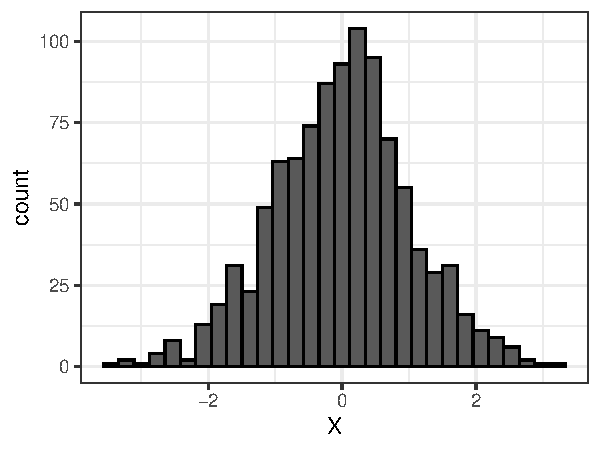
\includegraphics{figures-and-tables/normal-histogram.pdf}
\caption{A sample of 1000 standard normal random variables.}
\label{fig:std-norm-hist}
\end{figure}

\item[(b)] The histogram looks bell-shaped, as one would expect.
\end{enumerate}

\end{sol}


\begin{prob} \textbf{Data analysis: Diamonds.} \\

\noindent Consider the \texttt{diamonds} dataset built into \texttt{ggplot2}, whose first few rows are shown below.

\begin{table}[!h]

\caption{\label{tab:diamonds-data}First five rows of \texttt{diamonds} data.}
\centering
\begin{tabular}[t]{rlllrrrrrr}
\toprule
carat & cut & color & clarity & depth & table & price & x & y & z\\
\midrule
0.23 & Ideal & E & SI2 & 61.5 & 55 & 326 & 3.95 & 3.98 & 2.43\\
0.21 & Premium & E & SI1 & 59.8 & 61 & 326 & 3.89 & 3.84 & 2.31\\
0.23 & Good & E & VS1 & 56.9 & 65 & 327 & 4.05 & 4.07 & 2.31\\
0.29 & Premium & I & VS2 & 62.4 & 58 & 334 & 4.20 & 4.23 & 2.63\\
0.31 & Good & J & SI2 & 63.3 & 58 & 335 & 4.34 & 4.35 & 2.75\\
\bottomrule
\end{tabular}
\end{table}


\begin{enumerate}
\item[(a)] Create a histogram of the diamond price, and comment on its shape.
\item[(b)] Create a table of average price by diamond cut, and comment on any trends.
\item[(c)] Run a linear regression of \texttt{price} on \texttt{carat}, and print a table of the regression summary. Comment on the results.
\end{enumerate}

\end{prob}

\begin{sol}

\begin{enumerate}
  \item[(a)] Figure~\ref{fig:price-hist} shows the distribution of diamond price. We see that the distribution has a long right tail.
  
  \begin{figure}[h!]
    \centering
    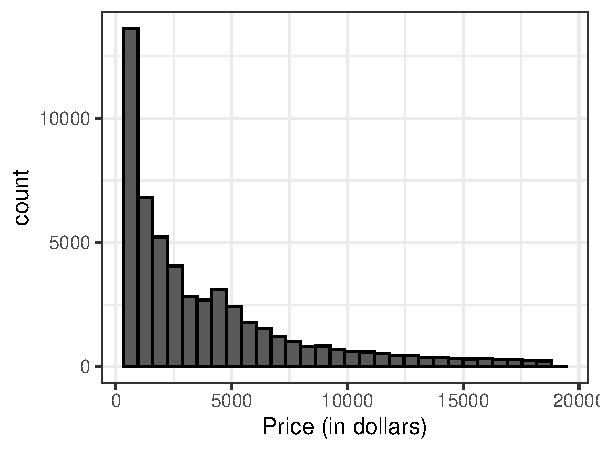
\includegraphics{figures-and-tables/price-histogram.pdf}
    \caption{The distribution of \texttt{price} in the \texttt{diamonds} dataset.}
    \label{fig:price-hist}
  \end{figure}

  \item[(b)] Table~\ref{tab:diamond-price-by-cut} shows the mean diamond price by cut. Surprisingly, the mean diamond price appears to \textit{decrease} as cut improves!
  \begin{table}[!h]

\caption{\label{tab:diamond-price-by-cut}Mean diamond price by cut.}
\centering
\begin{tabular}[t]{lr}
\toprule
Cut & Mean Price (\$)\\
\midrule
Fair & 4358.76\\
Good & 3928.86\\
Very Good & 3981.76\\
Premium & 4584.26\\
Ideal & 3457.54\\
\bottomrule
\end{tabular}
\end{table}


  \item[(c)] Table~\ref{tab:regression-output} shows the regression output. It appears that the carat of a diamond has an extremely significant impact on its price.
  
  
% Table created by stargazer v.5.2.3 by Marek Hlavac, Social Policy Institute. E-mail: marek.hlavac at gmail.com
% Date and time: Thu, Aug 18, 2022 - 18:47:04
\begin{table}[!htbp] \centering 
  \caption{Results of regressing price on carat.} 
  \label{tab:regression-output} 
\begin{tabular}{@{\extracolsep{5pt}}lc} 
\\[-1.8ex]\hline 
\hline \\[-1.8ex] 
 & \multicolumn{1}{c}{\textit{Dependent variable:}} \\ 
\cline{2-2} 
\\[-1.8ex] & price \\ 
\hline \\[-1.8ex] 
 carat & 7,756.426$^{***}$ \\ 
  & (14.067) \\ 
  & \\ 
 Constant & $-$2,256.361$^{***}$ \\ 
  & (13.055) \\ 
  & \\ 
\hline \\[-1.8ex] 
Observations & 53,940 \\ 
R$^{2}$ & 0.849 \\ 
Adjusted R$^{2}$ & 0.849 \\ 
Residual Std. Error & 1,548.562 (df = 53938) \\ 
F Statistic & 304,050.900$^{***}$ (df = 1; 53938) \\ 
\hline 
\hline \\[-1.8ex] 
\textit{Note:}  & \multicolumn{1}{r}{$^{*}$p$<$0.1; $^{**}$p$<$0.05; $^{***}$p$<$0.01} \\ 
\end{tabular} 
\end{table} 

\end{enumerate}
    

\end{sol}

\end{document}